\section{Background}
\label{sec:background}

Before you start the lab, we strongly recommend you read this section. 

\subsection{Your Tools}


\subsubsection{Hardware}

You have a Raspberry Pi.
The Raspberry PI 3 Module B+ contains 4 Cortex-A53 cores, which is Armv8-A architecture.
It supports both 32-bit Armv8-A (also called aarch32) and 64-bit Armv8-A (also called aarch64) architecture.
The official kernel is compiled as 32-bit Armv8-A architecture.

\subsubsection{Boot directory}

In the SD card file system, it contains a directory, "boot", which stores the important configurations ("config.txt"), kernel ("kernel.img" or "kernel7.img"), device tree files ("*.dtb"), and etc.
In this lab, you should replace the \textbf{kernel} and necessary \textbf{device tree files}. You may use the configurations to support HDMI.

\subsubsection{Source Code of Linux Kernel}

In the following instructions, you should download the source codes of the Linux kernel, and compile them.
You can download it here (version 4.14):

\begin{lstlisting}
git clone http://github.com/raspberrypi/linux -b rpi-4.14.y
\end{lstlisting}

\subsubsection{(Optional) Cross-compile Tools}

You can compile the kernel on a virtual machine, then copy kernel image, dtb files, and modules into the disk.
However, since you want to compile a \texttt{Arm}-based kernel, and your virtual machine is \texttt{x86} architecture, you must use the \textbf{Cross Compile} tools to achieve your goal.

Here is the source of the tools:

\begin{lstlisting}
git clone git://github.com/raspberrypi/tools.git
\end{lstlisting}

When you \texttt{make} the kernel in 64-bit Ubuntu, you must configure the position of your compilation tools (\texttt{CROSS\_COMPILE}).



\subsection{Armv8-A Exception Levels}

In Figure~\ref{fig:armel}, Armv8-A define four exception levels (EL0 - EL3) with different privilege, and the higher number indicates the higher privilege.
The components with higher-level privileges can access the source (e.g., memory and registers) of lower-level privileges.
Detailed usage of exception levels are listed as follows:

\begin{itemize}
	\item EL0: used for user applications, such as a game.
	\item EL1: used for the kernel, including the GPU driver, virtual address management, etc.
	\item EL2: used for the hypervisor, also called as virtualization layer.
	\item EL3: used for secure monitor (not used in our defense).
\end{itemize}

\begin{figure}[htb]
	\centering
	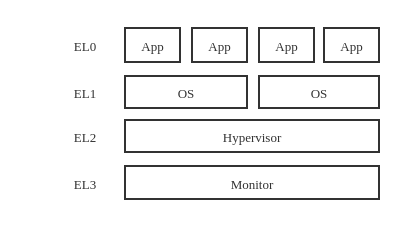
\includegraphics[width=0.6\linewidth]{el.png}
	\caption{Armv8-A Exception Level, source from
		https://developer.arm.com/documentation/den0024/a/Fundamentals-of-ARMv8}
	\label{fig:armel}
\end{figure}


Generally, if the lower-level user wants to use the feature in higher exception levels (for instance, an application requires a memory region to place the data).
It will generate an exception (this is not a bad word), which will be handled by the corresponding exception handler in the higher ELs.
Usually, such procedure is safe, because the normal system should not leave a "backdoor" (such as providing a root privilege for the user) in the exception handlers. However, the \TheName{} leverages the debugging mechanism to jump to higher exception levels and execute arbitrary codes which do not exist in any exception handlers. Therefore, we regard the behavior as an "attack".

In this lab, we assume the attacker controls EL0 \& EL1, and we design a defense on EL2.
Note that the EL1 attacker cannot directly access the resource in EL2 (You can try to read an EL2 register in a kernel module, and find the module is crashed). 


\begin{figure}[htb]
	\centering
	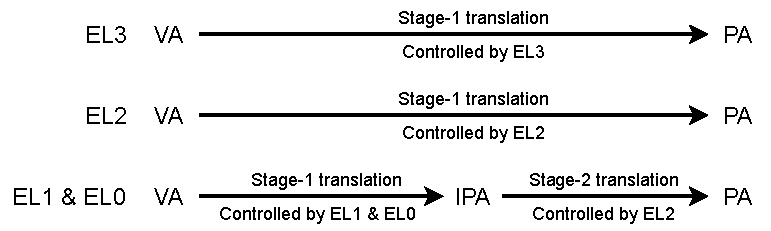
\includegraphics[width=0.8\linewidth]{s2trans_back.pdf}
	\caption{The mechanism of address translation in Armv8-A}
	\label{fig:armat}
\end{figure}

\subsection{Armv8-A Address Translation}

For memory management, Armv8-A defines 3 types of address: the virtual address (\texttt{VA}),
the intermediate physical address (\texttt{IPA}) and the physical address
(\texttt{PA}).
Armv8-A defines Stage-1 address translation for each exception level. 
Moreover, Armv8-A introduces an additional address translation for translation regime in EL0 \& EL1, called the State-2 translation, which is controlled by EL2.
As described in
Figure~\ref{fig:armat}, the VA in EL0 \& EL1 must be first translated into an IPA before reaching a PA.

If the IPA to PA is failed, the translation will not reach a correct result.
Therefore, in this lab, we can leverage the Stage-2 translation to control the access of the physical memory regions. Specifically, the region mapped to the debug registers.
